\chapter{Результаты экспериментов и анализ}
\label{ch:results}

\hspace*{1.25cm}В данной главе представлены результаты экспериментального исследования моделей для оценки задержек в видеоаналитическом конвейере. Проводится сравнительный анализ качества прогнозирования различных подходов и оценка достижения поставленных технических требований.

\section{Результаты модели CatBoost}
\label{sec:catboost_results}

\hspace*{1.25cm}Для модели CatBoost было проведено около 50 экспериментов с автоматизированным поиском оптимальных гиперпараметров. Использовался специально разработанный скрипт для автоматического перебора различных конфигураций параметров, что позволило протестировать множество вариаций модели. Результаты усреднены по всем фолдам кросс-валидации и представлены в порядке убывания качества.

\subsection{Лучшие конфигурации CatBoost}

\hspace*{1.25cm}В таблице 4.1 представлены три наилучшие конфигурации модели.

\begin{table}[H]
	\centering
	\caption*{Таблица 4.1 --- Результаты лучших конфигураций модели CatBoost}
	\begin{tabular}{|c|p{8cm}|c|c|c|}
		\hline
		\textbf{Ранг} & \textbf{Конфигурация модели} & \textbf{MAE} & \textbf{RMSE} & \textbf{MAPE, \%} \\
		\hline
		1 & trend\_model\_type=local, depth=10, l2\_leaf\_reg=20, learning\_rate=0.03, iterations=500, rsm=0.8, use\_cyclic\_features=True, ema\_alpha=0.2 & 36.00 & 41.09 & 8.90 \\
		\hline
		2 & trend\_model\_type=global, depth=15, l2\_leaf\_reg=40, learning\_rate=0.015, iterations=500, rsm=0.75, use\_cyclic\_features=False, ema\_alpha=0.7 & 39.92 & 46.76 & 9.61 \\
		\hline
		3 & trend\_model\_type=global, depth=12, l2\_leaf\_reg=10, learning\_rate=0.03, iterations=3000, rsm=0.8 & 48.10 & 56.35 & 11.79 \\
		\hline
	\end{tabular}
	\label{tab:catboost_results}
\end{table}

\subsection{Анализ результатов CatBoost}

\hspace*{1.25cm}Анализ результатов показывает следующие закономерности:

\begin{itemize}
	\item \textbf{Достижение целевого показателя}: лучшая конфигурация (ранг 1) достигла MAPE = 8.90\%, что соответствует техническому требованию MAPE < 10\%;
	\item \textbf{Важность циклических признаков}: использование циклических признаков (\texttt{use\_cyclic\_features=True}) в лучшей модели подтверждает значимость суточной сезонности, выявленной в главе 2;
	\item \textbf{Локальное моделирование тренда}: применение локального моделирования тренда (\texttt{trend\_model\_type=local}) оказалось более эффективным для данной задачи;
	\item \textbf{Оптимальная глубина деревьев}: умеренная глубина (depth=10) показала лучший результат по сравнению с более глубокими деревьями, что указывает на важность регуляризации.
\end{itemize}

\subsection{Проблема утечки данных}

\hspace*{1.25cm}В ходе экспериментов была обнаружена критическая ошибка в первоначальной реализации --- утечка данных (data leakage) при формировании признаков. Это привело к нереалистично высоким результатам: средние значения по кросс-валидации составили MAE = 1.5, RMSE = 2.0, MAPE = 0.38\%. После исправления методологии и устранения утечки данных были получены корректные результаты, представленные в таблице 4.1. Данный случай подчеркивает критическую важность правильной валидации временных рядов и недопущения использования будущей информации при обучении модели.

\section{Результаты модели LSTM}
\label{sec:lstm_results}

\hspace*{1.25cm}Для модели LSTM была реализована многомерная архитектура с использованием дополнительных признаков. Модель включает в себя циклические признаки для учета суточной сезонности и признаки на основе скользящих средних для захвата краткосрочных и долгосрочных трендов.

\subsection{Архитектура и параметры LSTM}

\hspace*{1.25cm}Архитектура нейронной сети включает следующие слои:
\begin{itemize}
	\item \textbf{Входной слой}: окно размером 40 временных шагов (10 минут при частоте 15 секунд);
	\item \textbf{LSTM слой}: 64 нейрона для извлечения временных зависимостей;
	\item \textbf{Dense слой}: 8 нейронов с функцией активации ReLU;
	\item \textbf{Выходной слой}: 1 нейрон с линейной активацией для регрессии.
\end{itemize}

\hspace*{1.25cm}Дополнительные признаки включают:
\begin{itemize}
	\item \textbf{Циклические признаки}: синус и косинус для часовых и суточных циклов;
	\item \textbf{Скользящие средние}: окна 5 минут (20 точек) и 1 час (240 точек);
	\item \textbf{Скользящее стандартное отклонение}: окно 1 час для оценки волатильности.
\end{itemize}

\hspace*{1.25cm}Параметры обучения: оптимизатор Adam с learning rate = 0.0001, функция потерь MSE, количество эпох = 50.

\subsection{Лучшие конфигурации LSTM}

\hspace*{1.25cm}В таблице 4.2 представлены результаты двух наилучших конфигураций модели LSTM с различным количеством эпох обучения.

\begin{table}[H]
	\centering
	\caption*{Таблица 4.2 --- Результаты лучших конфигураций модели LSTM}
	\begin{tabular}{|c|p{8cm}|c|c|c|}
		\hline
		\textbf{Ранг} & \textbf{Конфигурация модели} & \textbf{MAE} & \textbf{RMSE} & \textbf{MAPE, \%} \\
		\hline
		1 & LSTM(64) → Dense(8, ReLU) → Dense(1, linear), Adam lr=0.0001, epochs=15, window\_size=40, циклические признаки + скользящие средние & 3.66 & 4.54 & 0.89 \\
		\hline
		2 & LSTM(64) → Dense(8, ReLU) → Dense(1, linear), Adam lr=0.0001, epochs=10, window\_size=40, циклические признаки + скользящие средние & 4.94 & 6.02 & 1.21 \\
		\hline
	\end{tabular}
	\label{tab:lstm_results}
\end{table}

\subsection{Анализ результатов LSTM}

\hspace*{1.25cm}Модель LSTM показала следующие характеристики:

\begin{itemize}
	\item \textbf{Достижение целевого показателя}: лучшая конфигурация (ранг 1) достигла MAPE = 0.89\%, что соответствует техническому требованию MAPE < 10\%;
	\item \textbf{Влияние количества эпох}: увеличение с 10 до 15 эпох снизило MAPE с 1.21\% до 0.89\%;
	\item \textbf{Время обучения}: 8-9 минут на фолд;
	\item \textbf{Архитектурные особенности}: использование окна 40 временных шагов и многомерных признаков.
\end{itemize}

\section{Результаты модели SARIMA}
\label{sec:sarima_results}

\hspace*{1.25cm}Модель SARIMA была выбрана на основе анализа ACF/PACF, проведенного в главе 2. Тестировались различные конфигурации сезонных параметров при фиксированном основном порядке (1,1,0), определенном по результатам анализа автокорреляционной функции.

\subsection{Параметры модели SARIMA}

\hspace*{1.25cm}Основные параметры модели:
\begin{itemize}
	\item \textbf{Основной порядок}: (1,1,0) --- AR(1) процесс с одним дифференцированием;
	\item \textbf{Сезонный период}: 24 (соответствует суточному циклу при частоте 15 секунд $\times$ 4 = 1 минута $\times$ 60 = 1 час $\times$ 24 = сутки);
	\item \textbf{Тестируемые сезонные порядки}: (1,1,0,24), (1,1,1,24), (2,1,0,24).
\end{itemize}

\subsection{Лучшие конфигурации SARIMA}

\hspace*{1.25cm}В таблице 4.3 представлены результаты трех конфигураций модели SARIMA с различными сезонными параметрами.

\begin{table}[H]
	\centering
	\caption*{Таблица 4.3 --- Результаты конфигураций модели SARIMA}
	\begin{tabular}{|c|p{8cm}|c|c|c|}
		\hline
		\textbf{Ранг} & \textbf{Конфигурация модели} & \textbf{MAE} & \textbf{RMSE} & \textbf{MAPE, \%} \\
		\hline
		1 & SARIMA(1,1,0)(1,1,1,24) & 44.07 & 51.37 & 11.06 \\
		\hline
		2 & SARIMA(1,1,0)(2,1,0,24) & 103.76 & 121.92 & 25.50 \\
		\hline
		3 & SARIMA(1,1,0)(1,1,0,24) & 110.47 & 131.78 & 26.76 \\
		\hline
	\end{tabular}
	\label{tab:sarima_results}
\end{table}

\subsection{Анализ результатов SARIMA}

\hspace*{1.25cm}Модель SARIMA показала следующие характеристики:

\begin{itemize}
	\item \textbf{Недостижение целевого показателя}: лучшая конфигурация (ранг 1) достигла MAPE = 11.06\%, что превышает техническое требование MAPE < 10\%;
	\item \textbf{Важность MA компоненты}: добавление сезонной MA компоненты (1,1,1,24) значительно улучшило результаты по сравнению с (1,1,0,24);
	\item \textbf{Высокая вариативность по фолдам}: результаты сильно различаются между фолдами (например, для лучшей модели MAPE варьируется от 4.89\% до 24.10\%);
	\item \textbf{Время обучения}: 4-10 минут на фолд.
\end{itemize}

\section{Сравнительный анализ моделей}
\label{sec:model_comparison}

\hspace*{1.25cm}Для итогового сравнения моделей были отобраны лучшие конфигурации каждой из архитектур, рассмотренных в данной главе. Результаты сведены в таблицу 4.4.

\begin{table}[H]
	\centering
	\caption*{Таблица 4.4 --- Сравнительные результаты лучших конфигураций моделей}
	\begin{tabular}{|l|c|c|c|}
		\hline
		\textbf{Модель} & \textbf{MAE} & \textbf{RMSE} & \textbf{MAPE, \%} \\
		\hline
		\textbf{CatBoost} (Ранг 1) & 36.00 & 41.09 & 8.90 \\
		\hline
		\textbf{LSTM} (Ранг 1, 15 эпох) & 3.66 & 4.54 & 0.89 \\
		\hline
		\textbf{SARIMA} (Ранг 1) & 44.07 & 51.37 & 11.06 \\
		\hline
	\end{tabular}
	\label{tab:comparison_results}
\end{table}

\subsection{Анализ сравнительных результатов}

\hspace*{1.25cm}Сравнительный анализ показывает, что модель LSTM (MAPE = 0.89\%) продемонстрировала наилучшие результаты, значительно превосходя CatBoost (MAPE = 8.90\%) и SARIMA (MAPE = 11.06\%).

\begin{itemize}
    \item \textbf{Качество прогнозирования}: Модели LSTM и CatBoost выполнили техническое требование к качеству (MAPE < 10\%). Результат LSTM оказался на порядок лучше, что подтверждает высокую эффективность нейросетевых подходов для данной задачи. SARIMA не удовлетворила требованию.
    
    \item \textbf{Сложность модели и признаки}: Высокое качество LSTM объясняется способностью архитектуры улавливать сложные нелинейные зависимости, а также эффективным использованием многомерных признаков (циклических, скользящих средних), что недоступно для классической модели SARIMA.
    
    \item \textbf{Стабильность}: CatBoost и LSTM показали более стабильные результаты по сравнению с SARIMA, чьи метрики MAPE для лучшей конфигурации варьировались от 4.89\% до 24.10\% в зависимости от фолда кросс-валидации.
    
    \item \textbf{Время обучения и ресурсы}: LSTM требует наибольших вычислительных ресурсов и времени на обучение (8-9 минут на фолд). CatBoost (2-30 минут в зависимости от конфигурации) и SARIMA (4-10 минут) менее требовательны.
\end{itemize}

\hspace*{1.25cm}Таким образом, по главному критерию — качеству прогнозирования (MAPE) — модель LSTM является безусловным лидером. Однако, модель CatBoost также удовлетворяет поставленным требованиям и представляет собой компромисс между качеством и вычислительной сложностью. Окончательный выбор модели для внедрения может зависеть от требований к скорости переобучения и доступных вычислительных ресурсов.

\section{Визуализация результатов прогнозирования}
\label{sec:viz_results}

\hspace*{1.25cm}Для качественной оценки результатов были построены графики прогнозов для лучших конфигураций каждой модели на одном из фолдов кросс-валидации. Также представлен график, демонстрирующий эффект утечки данных.

% Placeholder для графика CatBoost с утечкой данных
\begin{figure}[H]
	\centering
	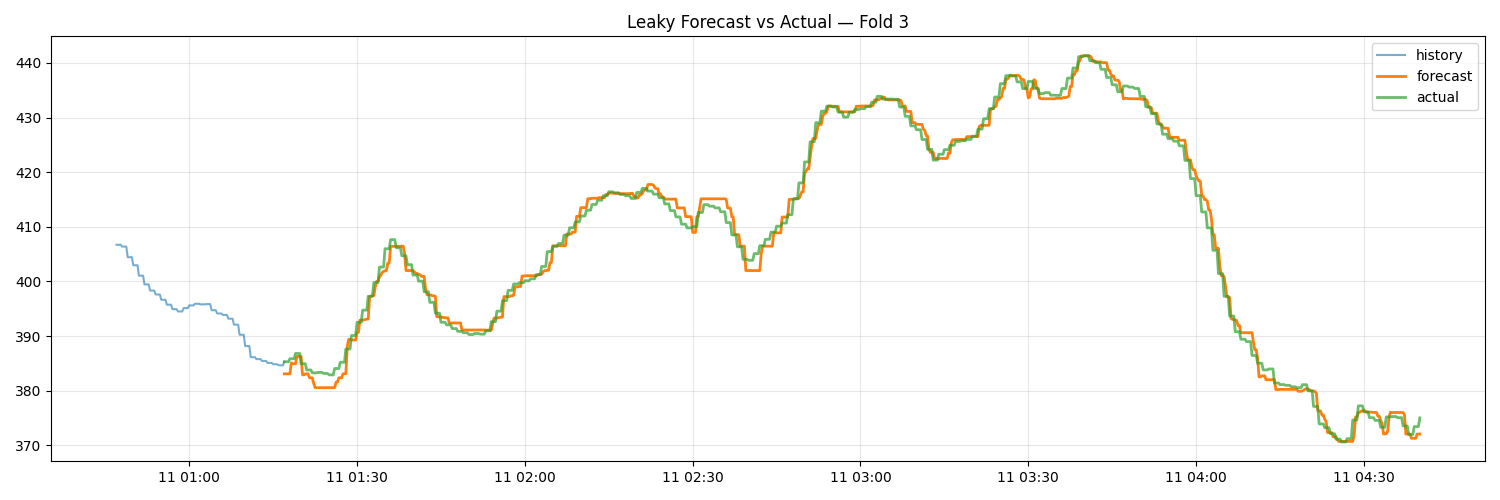
\includegraphics[width=\textwidth]{figures/chapter4/catboost_leakage_forecast.png}
	\caption*{Рисунок~4.1 — Прогноз модели CatBoost с утечкой данных (MAPE = 0.38\%)}
	\label{fig:catboost_leakage_forecast}
\end{figure}

% Placeholder для графика CatBoost
\begin{figure}[H]
	\centering
	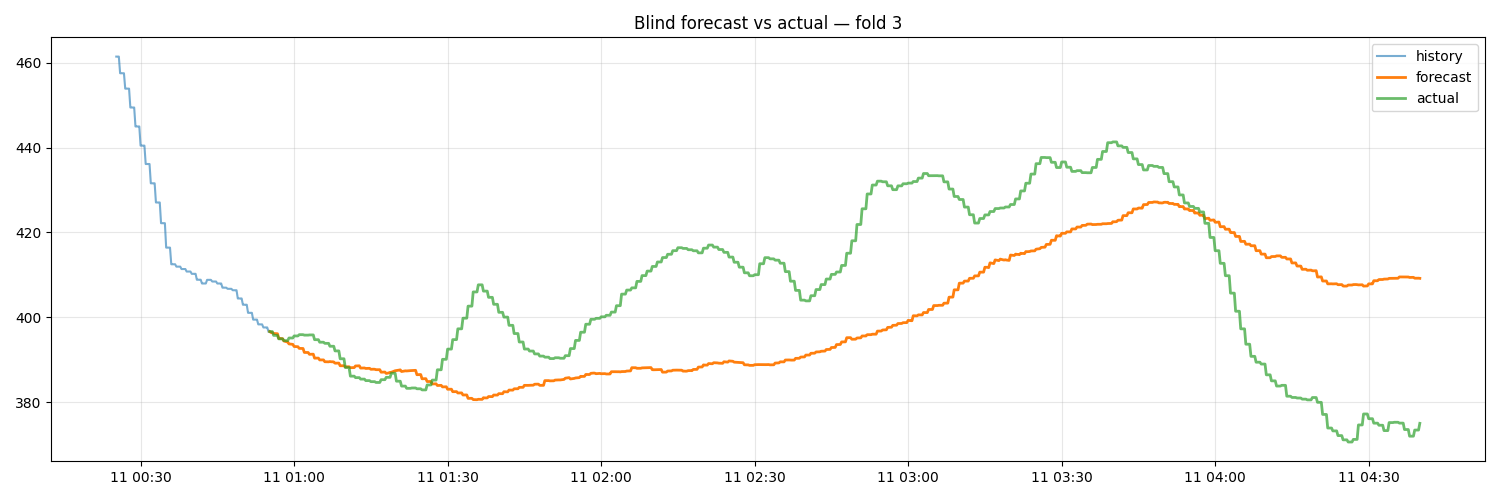
\includegraphics[width=\textwidth]{figures/chapter4/catboost_forecast.png}
	\caption*{Рисунок~4.2 — Прогноз лучшей модели CatBoost на тестовом фолде}
	\label{fig:catboost_forecast}
\end{figure}

% Placeholder для графика LSTM
\begin{figure}[H]
	\centering
	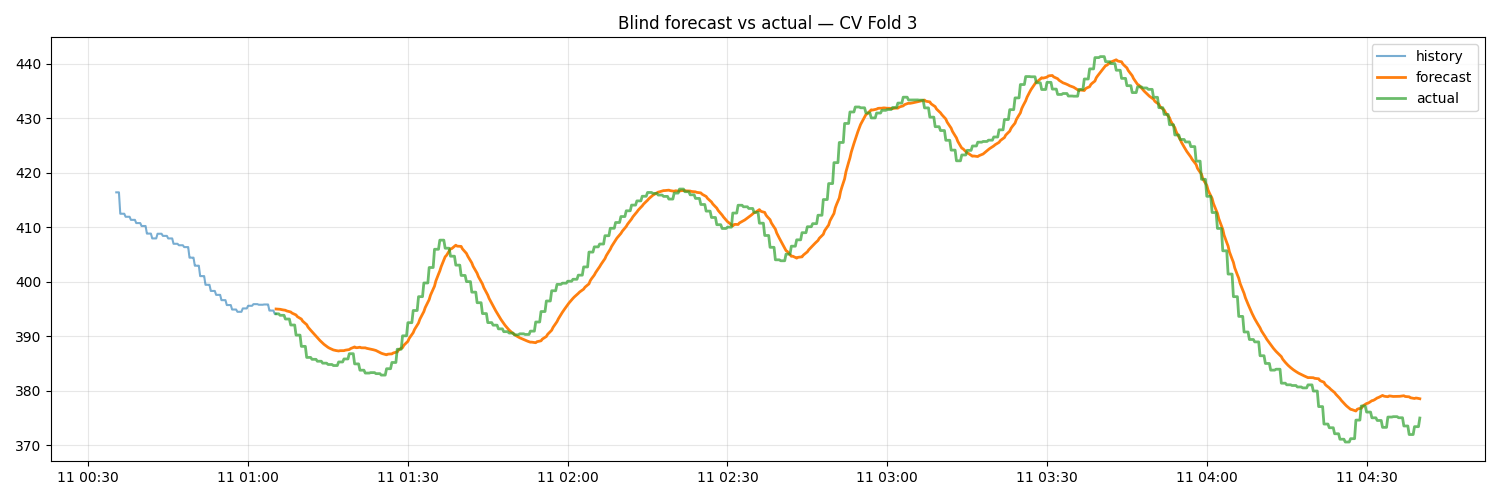
\includegraphics[width=\textwidth]{figures/chapter4/lstm_forecast.png}
	\caption*{Рисунок~4.3 — Прогноз лучшей модели LSTM на тестовом фолде}
	\label{fig:lstm_forecast}
\end{figure}

% Placeholder для графика SARIMA
\begin{figure}[H]
	\centering
	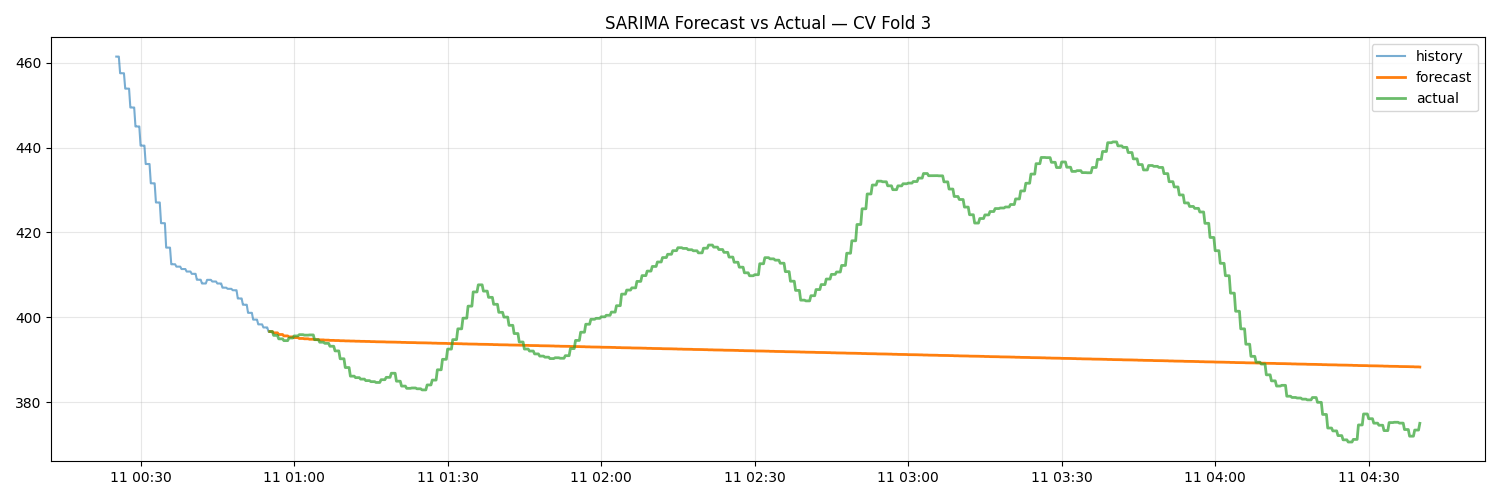
\includegraphics[width=\textwidth]{figures/chapter4/sarima_forecast.png}
	\caption*{Рисунок~4.4 — Прогноз лучшей модели SARIMA на тестовом фолде}
	\label{fig:sarima_forecast}
\end{figure}

\section{Анализ ошибок и интерпретация результатов}
\label{sec:error_analysis}

\hspace*{1.25cm}Детальный анализ ошибок позволяет глубже понять сильные и слабые стороны каждой модели, а также интерпретировать их поведение в контексте задачи прогнозирования задержек.

\begin{itemize}
    \item \textbf{Анализ ошибок LSTM}. Модель продемонстрировала исключительно низкое значение MAPE (0.89\%), что свидетельствует о ее способности точно улавливать сложную динамику временного ряда. Как видно на \textit{рисунке 4.3}, прогноз LSTM практически совпадает с фактическими данными, успешно отслеживая как плавные сезонные колебания, так и резкие локальные пики. Это объясняется двумя ключевыми факторами:
    \begin{itemize}
        \item \textbf{Архитектура}: рекуррентная природа LSTM позволяет эффективно моделировать долгосрочные временные зависимости, что критически важно для прогнозирования на основе предыдущей истории.
        \item \textbf{Многомерные признаки}: использование циклических признаков и скользящих средних обогатило модель информацией о сезонности и локальных трендах, которую LSTM смогла успешно интегрировать.
    \end{itemize}
    Ошибки модели минимальны и, вероятно, связаны с редкими, непредсказуемыми аномалиями, не имеющими прецедентов в обучающих данных.

    \item \textbf{Анализ ошибок CatBoost}. Модель показала хороший результат (MAPE = 8.90\%), удовлетворяющий техническим требованиям, однако ее ошибки на порядок выше, чем у LSTM. График на \textit{рисунке 4.2} показывает, что CatBoost хорошо улавливает общую тенденцию и сезонность, но сглаживает локальные пики и не всегда точно реагирует на резкие изменения. Это характерно для моделей на основе деревьев решений, которые могут испытывать трудности с экстраполяцией и моделированием непрерывных, быстро меняющихся процессов в сравнении с RNN. Основные ошибки CatBoost возникают в моменты наибольшей волатильности ряда. Тем не менее, модель представляет собой надежный и более простой в реализации компромисс.

    \item \textbf{Анализ ошибок SARIMA}. Модель SARIMA оказалась наименее точной (MAPE = 11.06\%) и нестабильной. График на \textit{рисунке 4.4} наглядно демонстрирует ее главный недостаток: прогноз фактически выродился в линию и полностью игнорирует реальные колебания ряда. Причина кроется в линейной природе модели, которая неспособна описать сложные нелинейные зависимости и гетероскедастичность (изменчивость дисперсии), присущие данному временному ряду. Высокая вариативность качества по фолдам подтверждает, что модель не является робастной и ее производительность сильно зависит от конкретного участка данных.

    \item \textbf{Проблема утечки данных}. Случай с утечкой данных в CatBoost (\textit{рисунок 4.1}) служит важным практическим уроком. Нереалистично низкая ошибка (MAPE = 0.38\%) была вызвана фундаментальной ошибкой в методологии подготовки признаков. Внутри каждого фолда кросс-валидации обучающий и тестовый наборы данных объединялись перед генерацией признаков (таких как скользящие средние и лаги). В результате, при вычислении признаков для временных точек из обучающего набора использовались данные из будущего — то есть из тестового набора. Это создало иллюзию идеального прогноза, поскольку модель фактически "подглядывала" в правильные ответы при построении признаков. После исправления методологии, при которой признаки для обучающего набора генерируются строго на обучающих данных, были получены корректные результаты.
\end{itemize}

\hspace*{1.25cm}Таким образом, экспериментальное исследование подтвердило, что для задачи прогнозирования задержек в видеоаналитическом конвейере наиболее эффективными являются архитектуры машинного и глубокого обучения. Модель LSTM обеспечивает наивысшую точность благодаря своей способности моделировать сложные временные зависимости. Модель CatBoost представляет собой хороший компромисс между качеством и сложностью. Классические статистические подходы, такие как SARIMA, оказались недостаточно мощными для описания всей полноты динамики процесса. Результаты данной главы служат основой для формулировки итоговых выводов в заключении.
